%!TEX root = <main.tex>
\section{Optimizations}\label{sec:optimizer}

In this section we explain \textit{incremental inference} and the two \textit{approximate inference} approaches, \textit{projective field thresholding} and \textit{adaptive drill-down} in detail.
In \system~ these optimizations are applied on top of the current dominant approach of performing CNN inference on batches of images where each image corresponds to an occluded instance of the original image.
Batched inference is important as it reduces per image inference time by amortizing the fixed overheads.
In our experiments we found that this simple optimization alone can give up to ~1.4X speedups on CPU environments and ~2X speedups on the GPU environment compared to the per image inference approach.
Finally we explain how \system~ configures it's internal system configurations for \textit{approximate inference}.

\subsection{Incremental Inference}\label{sec:inc_computation}

As explained earlier, occlusion experiments in it's naive form performs many redundant computations.
In order to avoid these redundancies, layers in a CNN have to be change aware and operate in an incremental manner i.e. reuse previous computations as much as possible and compute only the required ones.
In this section we focus on transformations that operate on a local spatial context (i.e. Convolution and Pooling) as other types either has no redundancies (global context transformations) or is trivial to make incremental (point transformations).
% We also explain incremental implementations of two other linear algebra operators, element-wise addition and depth-wise concatenation.
% The choice of CPUs vs GPUs for CNN inference also brings up new concerns for the batched implementation of these incremental transformations and we explain two version of implementations, one which is a naive implementation of batched incremental inference approach and the other a GPU optimized version.

\vspace{2mm}
\noindent \textbf{Incremental Convolution and Pooling.}


\begin{table}[t]
  \centering
  \caption{Additional symbols used in the Optimizations Section}
  \scalebox{0.8}{\begin{tabular}{p{2cm}p{7.5cm}}
    \toprule
    \textbf{Symbol} & \textbf{Meaning}\\
    \midrule \midrule
    $x^\mathcal{I}_\mathcal{P},y^\mathcal{I}_\mathcal{P}$ & Starting coordinates of the input patch\\
    \midrule
    $x^\mathcal{R}_\mathcal{P},y^\mathcal{R}_\mathcal{P}$ & Starting coordinates of the patch that needs to be read in for the transformation\\
    \midrule
    $x^\mathcal{O}_\mathcal{P},y^\mathcal{O}_\mathcal{P}$ & Starting coordinates of the output patch\\
    \midrule
    $H^\mathcal{I}_\mathcal{P},W^\mathcal{I}_\mathcal{P}$ & Height, and width of the input patch\\
   	\midrule
   	$H^\mathcal{R}_\mathcal{P},W^\mathcal{R}_\mathcal{P}$ & Height, and width of the patch that needs to be read in for the transformation\\
   	\midrule
   	$H^\mathcal{O}_\mathcal{P},W^\mathcal{O}_\mathcal{P}$ & Height, and width of the output patch\\
    \midrule
    $\tau$ & Projective field threshold\\
    \midrule
    $r_{drill-down}$ & Stage two drill-down fraction used in \textit{adaptive drill-down}\\
    \bottomrule
  \end{tabular}}
\label{table:optimizer_symbols}
\end{table}

In Section \ref{sec:preliminaries} we explained that both convolution and polling transformations can be cast into a form of applying a filter along the spatial dimensions of the input volume.
However, how each transformation operate along the depth dimension is different.
For our purpose we are interested in finding the propagation of the patches in the input through the consecutive layers and hence both these transformations can be treated similarly.
The coordinates and the dimensions (i.e. height and width) of the modified patch in the output volume caused by a modified patch in the input volume are determined by the coordinates and the dimensions of the input patch, sizes of the filter kernel ($H_\mathcal{K}$ and $W_\mathcal{K}$), padding values ($P_x$ and $P_y$), and the strides ($S_x$ and $S_y$).
For example consider simplified demonstration showing a cross-section of input and output in Figure \ref{fig:dimensions}.
We use a coordinate system whose origin is placed at the top left corner of the input.
A patch, marked in red, is placed on the input starting off at $x^\mathcal{I}_\mathcal{P}, y^\mathcal{I}_\mathcal{P}$ coordinates and has a height of $H^\mathcal{I}_\mathcal{P}$ and width of $W^\mathcal{I}_\mathcal{P}$.
The updated patch in the output starts off at $x^\mathcal{O}_\mathcal{P}, y^\mathcal{O}_\mathcal{P}$ and has a height of $H^\mathcal{O}_\mathcal{P}$ and width of $W^\mathcal{O}_\mathcal{P}$.
Note that due to the overlapping nature of filter positions, to compute the output patch, transformations have to read a slightly larger context than the updated patch. This read in context is shown by the blue shaded area in Figure \ref{fig:dimensions}.
The starting coordinates of this read-in patch are denoted by $x^\mathcal{R}_\mathcal{P}, y^\mathcal{R}_\mathcal{P}$ and the dimensions are denoted by $W^\mathcal{R}_\mathcal{P}, H^\mathcal{R}_\mathcal{P}$.
The relationship between the coordinates and dimensions can be expressed as follows:

\begin{figure}[t]
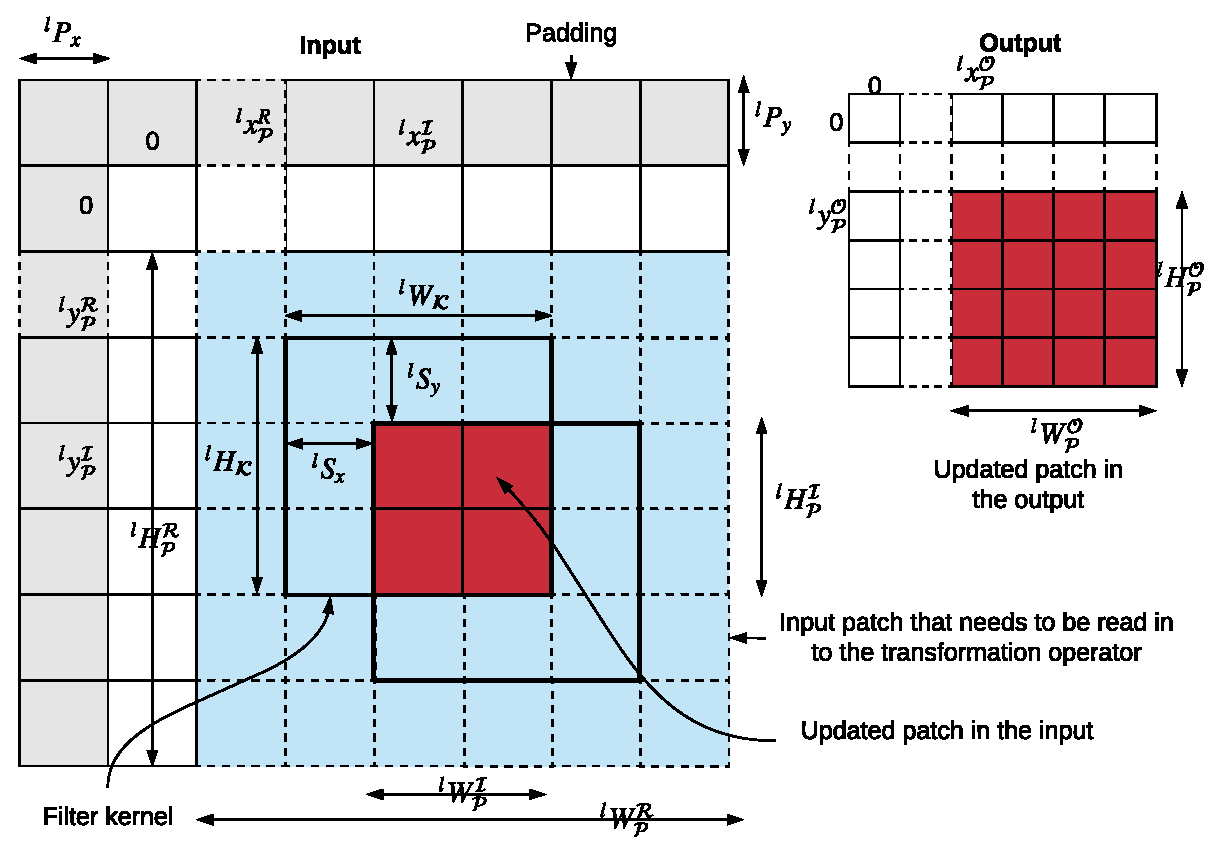
\includegraphics[width=\columnwidth]{images/dimensions}
\caption{Simplified representation of input and output patch coordinates and dimensions of Conv. and Pool transformations.}
\label{fig:dimensions}
\end{figure}

\begin{align}
\label{eqn:xcoordinate}
x^\mathcal{O}_\mathcal{P} =&~ max\big(\lceil (P_x + x^\mathcal{I}_\mathcal{P} - W_\mathcal{K} + 1)/S_x \rceil, 0\big)\\
\label{eqn:ycoordinate}
y^\mathcal{O}_\mathcal{P} =&~ max\big(\lceil (P_y + y^\mathcal{I}_\mathcal{P} - H_\mathcal{K} + 1)/S_y \rceil, 0\big)
\end{align}

\begin{align}
\label{eqn:patchwidth}
W^\mathcal{O}_\mathcal{P} =&~ min\big(\lceil (W^\mathcal{I}_\mathcal{P} + W_\mathcal{K} - 1)/S_x \rceil, W_{\mathcal{O}}\big)\\
\label{eqn:patchheight}
H^\mathcal{O}_\mathcal{P} =&~ min\big(\lceil (H^\mathcal{I}_\mathcal{P} + H_\mathcal{K} - 1)/S_y \rceil, H_{\mathcal{O}}\big)
\end{align}

\begin{align}
\label{eqn:xreadcoordinate}
x^\mathcal{R}_\mathcal{P} =&~ x^\mathcal{O}_\mathcal{P} \times S_x - P_x\\
\label{eqn:yreadcoordinate}
y^\mathcal{R}_\mathcal{P} =&~ y^\mathcal{O}_\mathcal{P} \times S_y - P_y
\end{align}

\begin{align}
\label{eqn:readpatchwidth}
W^\mathcal{R}_\mathcal{P} =&~ W_\mathcal{K} + (W^\mathcal{O}_\mathcal{P}-1) \times S_x\\
\label{eqn:readpatchheight}
H^\mathcal{R}_\mathcal{P} =&~ H_\mathcal{K} + (H^\mathcal{O}_\mathcal{P}-1) \times S_y
\end{align}


Equation \ref{eqn:xcoordinate} and \ref{eqn:ycoordinate} calculates the starting coordinates of the output patch.
Use of padding effectively shifts the coordinate system and therefore $P_x$ and $P_y$ values are added to correct it.
Due to the overlapping nature of filter kernels, the maximum affected span of the updated patch in the input will be increased by $W_\mathcal{K}-1$ and $H_\mathcal{K}-1$ amounts and hence needs to be subtracted from the input coordinates $x^\mathcal{I}_\mathcal{P}$ and $y^\mathcal{I}_\mathcal{P}$ (a filter of size $W_\mathcal{K}$ which is placed starting at $x^\mathcal{I}_\mathcal{P} - W_\mathcal{K} + 1$ will see the new change at $x^\mathcal{I}_\mathcal{P}$).
Dividing the above values by the stride values $S_x$ and $S_y$ and taking the \texttt{ceil} gives the starting coordinates of the output patch (essentially calculates the number of strides).
Towards the left side edge of the input, where the affected span of the input cannot be extended by $W_\mathcal{K}-1$ or $H_\mathcal{K}-1$ amounts this value will be negative.
Therefore the maximum of zero or the above value should be taken as the final.
Equation \ref{eqn:patchwidth} and \ref{eqn:patchheight} calculates the width and height of the output patches.
Similar to output coordinates calculations, the span of the input patch is increased by $W_\mathcal{K}-1$ and $H_\mathcal{K}-1$ amounts.
Dividing the above values by the stride values $S_x$ and $S_y$ and taking the \texttt{ceil} gives the width and height of the output patch.
Since the output patch cannot grow beyond the size of the output, minimum of the output dimension or the above value should be taken as the final.
Once the output patch coordinates and dimensions are calculated, it is straight forward to calculate the read-in patch coordinates as per Equations \ref{eqn:xreadcoordinate} and \ref{eqn:yreadcoordinate} and the dimensions as per Equations \ref{eqn:readpatchwidth} and \ref{eqn:readpatchheight}.

\begin{algorithm}
    \caption{Incremental Inference Transformation}\label{euclid}
    \label{alg:incinference}
    \begin{flushleft}
     \hspace*{4mm} \textbf{Input:} \\
     \hspace*{8mm} $T$ : \textit{Transformation}\\
     \hspace*{8mm} $\mathcal{I}$ : \textit{Pre-materialized input from original image}\\
     \hspace*{8mm} $[\mathcal{P^I}_1,...,\mathcal{P^I}_n]$ : \textit{Input patches}\\
     \hspace*{8mm} $[(x^\mathcal{I}_{\mathcal{P}_1},y^\mathcal{I}_{\mathcal{P}_1}),...,(x^\mathcal{I}_{\mathcal{P}_n},y^\mathcal{I}_{\mathcal{P}_n})]$ : \textit{Input patch coordinates}\\
     \hspace*{8mm} $W^\mathcal{I}_\mathcal{P},H^\mathcal{I}_\mathcal{P}$ : \textit{Input patch dimensions}
    \end{flushleft}

	\begin{flushleft}
     \hspace*{4mm} \textbf{Output:}\\
     \hspace*{8mm} $[\mathcal{P^O}_1,...,\mathcal{P^O}_n]$ : \textit{Output patches}\\
     \hspace*{8mm} $[(x^\mathcal{O}_{\mathcal{P}_1},y^\mathcal{O}_{\mathcal{P}_1}),...,(x^\mathcal{O}_{\mathcal{P}_n},y^\mathcal{O}_{\mathcal{P}_n})]$ : \textit{Output patch coordinates}\\
     \hspace*{8mm} $W^\mathcal{O}_\mathcal{P},H^\mathcal{O}_\mathcal{P}$ : \textit{Output patch dimensions}
    \end{flushleft}

    \begin{algorithmic}[1]
    \Procedure{IncrementalInference}{}
    \State \textit{Calculate} $[(x^\mathcal{O}_{\mathcal{P}_1},y^\mathcal{O}_{\mathcal{P}_1}),...,(x^\mathcal{O}_{\mathcal{P}_n},y^\mathcal{O}_{\mathcal{P}_n})]$ \textit{and} ($W^\mathcal{O}_\mathcal{P},H^\mathcal{O}_\mathcal{P}$)
    \State \textit{Calculate} $[(x^\mathcal{R}_{\mathcal{P}_1},y^\mathcal{R}_{\mathcal{P}_1}),...,(x^\mathcal{R}_{\mathcal{P}_n},y^\mathcal{R}_{\mathcal{P}_n})]$ \textit{and} ($W^\mathcal{R}_\mathcal{P},H^\mathcal{R}_\mathcal{P}$)
    \State \textit{Initialize} $\mathcal{R} \in \mathcal{\rm I\!R}^{\texttt{depth}(\mathcal{I}) \times H^\mathcal{R}_\mathcal{P} \times W^\mathcal{R}_\mathcal{P}}$

    \For{\texttt{i in [1,...,n]}}\label{alg:line:memcpy_loop}
    	\State $T_1 \gets \mathcal{I}[:,x^\mathcal{R}_{\mathcal{P}_i}:x^\mathcal{R}_{\mathcal{P}_i}+W^\mathcal{R}_\mathcal{P},y^\mathcal{R}_{\mathcal{P}_i}:y^\mathcal{R}_{\mathcal{P}_i}+H^\mathcal{R}_\mathcal{P}]$ 
    	\State $T_2 \gets \mathcal{P}_i \bm\circ_{(x^\mathcal{I}_{\mathcal{P}_i}-x^\mathcal{R}_{\mathcal{P}_i}),(y^\mathcal{I}_{\mathcal{P}_i}-y^\mathcal{R}_{\mathcal{P}_i})} T_1$
    	\State $R[i,:,:] \gets T_2$
    \EndFor

    \State $[\mathcal{P}^\mathcal{O}_1,...,\mathcal{P}^\mathcal{O}_n] \gets T(\mathcal{R})$
    \State \textbf{return} $[\mathcal{P}^\mathcal{O}_1,...,\mathcal{P}^\mathcal{O}_n]$, $[(x^\mathcal{O}_{\mathcal{P}_1},y^\mathcal{O}_{\mathcal{P}_1}),...,(x^\mathcal{O}_{\mathcal{P}_n},y^\mathcal{O}_{\mathcal{P}_n})],$
    \State \hspace*{20mm} ($W^\mathcal{O}_\mathcal{P},H^\mathcal{O}_\mathcal{P}$) 
    \EndProcedure
    \end{algorithmic}

    \vspace*{-2mm}
    \hrulefill
    
    \begin{flushleft}
     \hspace*{4mm} \textbf{Input:}\\
     \hspace*{8mm} $\mathcal{O}$ : \textit{Pre-materialized output from original image}\\
     \hspace*{8mm} $[\mathcal{P}^\mathcal{O}_1,...,\mathcal{P}^\mathcal{O}_n]$ : \textit{Output patches}\\
     \hspace*{8mm} $[(x^\mathcal{O}_{\mathcal{P}_1},y^\mathcal{O}_{\mathcal{P}_1}),...,(x^\mathcal{O}_{\mathcal{P}_n},y^\mathcal{O}_{\mathcal{P}_n})]$ : \textit{Output patch coordinates}\\
    \end{flushleft}

    \begin{flushleft}
     \hspace*{4mm} \textbf{Output:}\\
     \hspace*{8mm} $O\textrm'$ : \textit{Updated output}
    \end{flushleft}
	\begin{algorithmic}[1]
    \Procedure{IncrementalToFullProjection}{}
    \State \textit{Initialize} $\mathcal{O}\textrm' \in \mathcal{\rm I\!R}^{n \times \texttt{depth}(\mathcal{O}) \times \texttt{height}(\mathcal{P}^\mathcal{O}_1) \times \texttt{width}(\mathcal{P}^\mathcal{O}_1)}$
    \For{\texttt{i in [1,...,n]}}
    	\State $T \gets \texttt{copy}(O)$
    	\State $\mathcal{O}\textrm'[i,:,:] \gets \mathcal{P}^\mathcal{O}_i \bm\circ_{x^\mathcal{O}_{\mathcal{P}_i},y^\mathcal{O}_{\mathcal{P}_i}} T$
    \EndFor
    \State \textbf{return} $\mathcal{O}\textrm'$
    \EndProcedure

    \end{algorithmic}
\end{algorithm}

With all the geometric mappings defined, we now explain the complete incremental inference approach for a single transformation. Algorithm \ref{alg:incinference} presents it formally.
The \textproc{IncrementalInference} procedure takes in the original transformation $T$, pre-materialized input for $T$ corresponding to original image, a batch of updated patches and their geometric properties as input.
First it calculates geometric properties of the output and read-in patches.
A temporary input volume $R$ is initialized to hold the input patches with their read-in contexts.
The \textsc{for} loop iteratively populates $R$ with corresponding patches.
Finally $T$ is applied on $R$ to compute the output patches.
In a CNN which has multiple such transformations chained together, the outputs of the \textproc{IncrementalInference} procedure are fed as input again for the incremental inference of the next transformation along with the unchanged pre-materialized input corresponding to the new transformation.
However at a boundary of local context transformation and a global context transformation, such as in Conv. $\rightarrow$ Fully-Connected or Pool $\rightarrow$ Fully-Connected, full updated output has to be created as per \textproc{IncrementalToFullProjection} procedure instead of propagating only the updated patches.
The high-level steps taken by the end-to-end incremental inference approach can be summarized as follows:

\begin{enumerate}
	\item Take in CNN $f$, image $\mathcal{I}_{img}$, predicted class label $C$, occlusion patch $\mathcal{P}$, and stride $S$ for the $\mathcal{P}$ as input.
	\item Pre-materialize output of all the transformations in $f$ by feeding in $\mathcal{I}_{img}$.
	\item Calculate all possible $\mathcal{P}$ positions on $\mathcal{I}_{img}$.
	\item Prepare the occluded images ($\mathcal{I}^{x,y}_{img}$ s) corresponding to all positions.
	\item For batches of $\mathcal{I}^{x,y}_{img}$ as the input traverse the transformations in $f$ in a topological order and calculate the corresponding values of heatmap $M$.
	\begin{itemize}
		\item For local context transformation invoke \textproc{IncrementalInference}.
		\item For local context transformation that feeds in a global context transformation additionally invoke \textproc{IncrementalToFullProjection}
		\item For all others invoke the original transformation.
	\end{itemize}
	\item Return M as the final output.
\end{enumerate}


\begin{figure}[t]
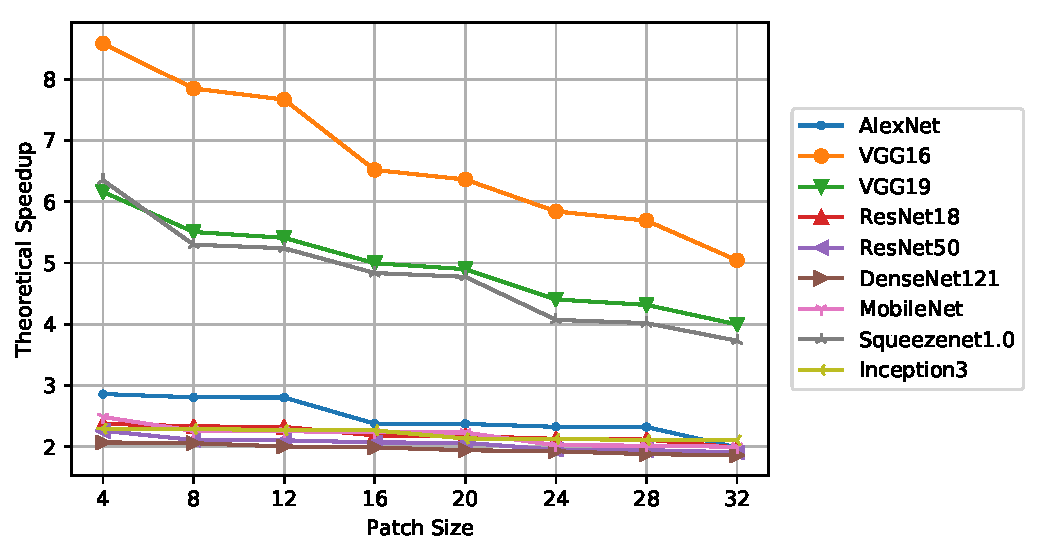
\includegraphics[width=\columnwidth]{images/redundancy_ratio}
\caption{Theoretical speedup for popular CNN architectures with \textit{incremental inference} when a square occlusion patch is placed on the center of the image.}
\label{fig:redundancy_ratio}
\end{figure}

We analyze the theoretical speedup that can be achieved with \textit{incremental inference} approach when a square occlusion patch is placed on the center\footnote{If the occlusion patch is placed towards to a corner of the input image the theoretical speedup will be slightly higher. But placing the occlusion patch on the center gives us a worst case estimate.} of the input image. Figure \ref{fig:redundancy_ratio} shows the results. VGG16 model results in the maximum theoretical speedup and DenseNet121 model has the lowest theoretical speedup. Most CNN architectures results in a theoretical speedup between 2-3. The theoretical speedup for a CNN with \textit{incremental inference} is determined by the characteristics of it's architecture such as number of layers, the sizes of the filter kernels, and the filter stride values.


\vspace{2mm}
\noindent \textbf{CPU versus GPU implementation concerns.}
Through our experiments we found that even though a straight-forward implementation of \textit{incremental inference} approach as shown in Algorithm \ref{alg:incinference} produces expected speedups for the CPU environment it performs poorly on the GPU environment.
The for loop on the line \ref{alg:line:memcpy_loop} of Algorithm \ref{alg:incinference} is essentially preparing the input for $T$ by copying values from one part of the memory to another sequentially.
This sequential operation becomes a bottleneck for the GPU implementation as it cannot exploit the available parallelism of the GPU efficiently.
To overcome this, we have extended PyTorch by adding a custom kernel written in CUDA language which performs the input preparation more efficiently by parallelly copying the memory regions for all items in the batch and then invoke the CNN transformation.

\vspace{2mm}
\noindent \textbf{Element-wise addition and depth-wise concatenation.}
Element-wise addition and depth-wise concatenation are two widely used linear algebra operators in CNNs.
Element-wise addition operator requires the two input volumes to have exact same dimensions and the depth-wise concatenation requires them to have same height and width dimensions.
Consider a situation for these operators as shown in Figure \ref{fig:la_operators} where the first input has incremental spatial update starting at $x^\mathcal{I}_{\mathcal{P}_1},y^\mathcal{I}_{\mathcal{P}_1}$ coordinates with dimensions of $H^\mathcal{I}_{\mathcal{P}_1}$ and $W^\mathcal{I}_{\mathcal{P}_1}$ and for the second input starting at $x^\mathcal{I}_{\mathcal{P}_2},y^\mathcal{I}_{\mathcal{P}_2}$ coordinates with dimensions of $H^\mathcal{I}_{\mathcal{P}_2}$ and $W^\mathcal{I}_{\mathcal{P}_2}$.
Then computing the coordinates and the dimensions of the output and read-in patches is essentially finding the bounding box for the two patches and can be expressed as follows:


\begin{figure}[t]
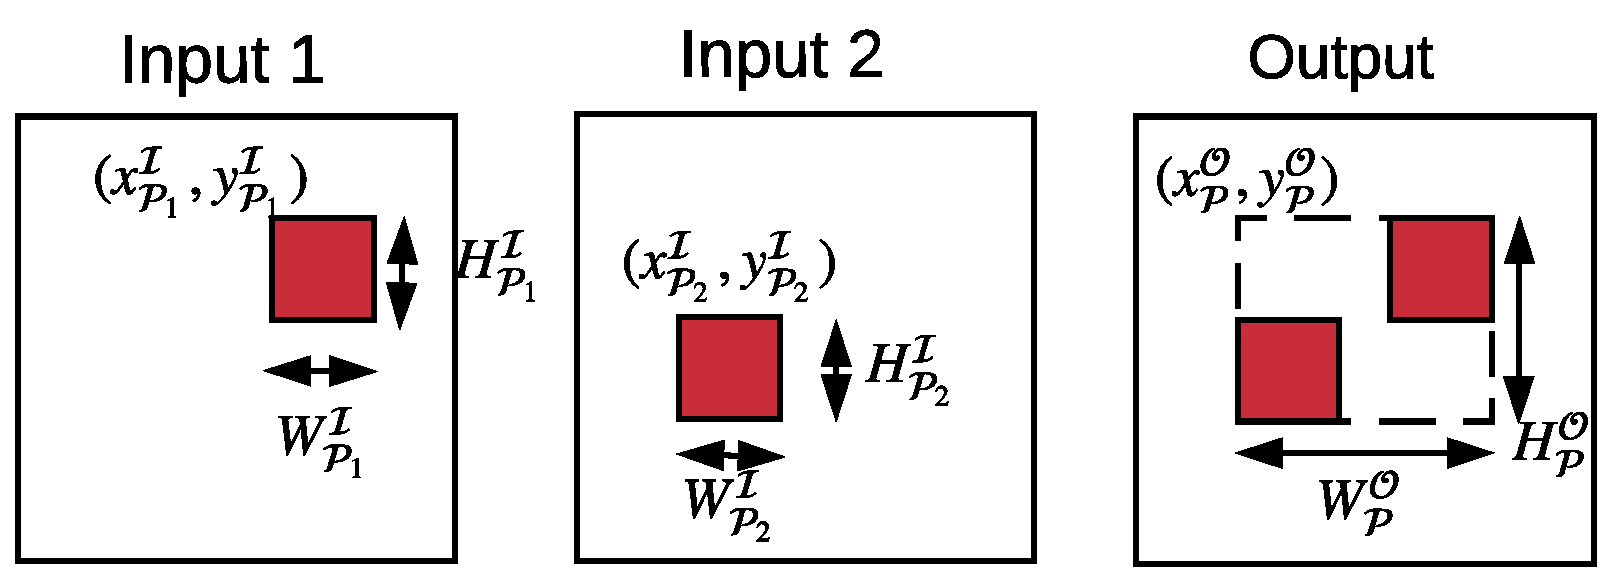
\includegraphics[width=\columnwidth]{images/la_operators}
\caption{Input-Output coordinate and dimension mapping for element-wise addition and depth-wise concatenation.}
\label{fig:la_operators}
\end{figure}

\begin{align}
\label{eqn:laxcoordinate}
x^\mathcal{O}_P = x^\mathcal{R}_\mathcal{P} =&~ \texttt{min}(x^\mathcal{I}_{\mathcal{P}_1},x^\mathcal{I}_{\mathcal{P}_2})\\
\label{eqn:laycoordinate}
y^\mathcal{O}_\mathcal{P} = y^\mathcal{R}_\mathcal{P} =&~ \texttt{min}(y^\mathcal{I}_{\mathcal{P}_1},y^\mathcal{I}_{\mathcal{P}_2})\\
\label{eqn:lapatchwidth}
W^\mathcal{O}_\mathcal{P} = W^\mathcal{R}_\mathcal{P} =&~ \texttt{max}(x^\mathcal{I}_{\mathcal{P}_1}+W^\mathcal{I}_{\mathcal{P}_1},x^\mathcal{I}_{\mathcal{P}_2}+W^\mathcal{I}_{\mathcal{P}_2})-\texttt{min}(x^\mathcal{I}_{\mathcal{P}_1},x^\mathcal{I}_{\mathcal{P}_2})\\
\label{eqn:lapatchheight}
H^\mathcal{O}_\mathcal{P} = H^\mathcal{R}_\mathcal{P} =&~ \texttt{max}(y^\mathcal{I}_{\mathcal{P}_1}+H^\mathcal{I}_{\mathcal{P}_1},y^\mathcal{I}_{\mathcal{P}_2}+H^\mathcal{I}_{\mathcal{P}_2})-\texttt{min}(y^\mathcal{I}_{\mathcal{P}_1},y^\mathcal{I}_{\mathcal{P}_2})
\end{align}


\subsection{Projective Field Thresholding}

Projective field \cite{le2017receptive, basiccnnoperations} of a CNN neuron is the local region (including the depth) of the output volume which is connected to it.
The term is borrowed from Neuroscience field where it is used to describe the spatiotemporal effects exerted by a retinal cell on all of the outputs of the neuronal circuitry \cite{de2011projective}.
For our work the notion of projective field is useful as it essentially determines the change propagation path for incremental changes.
The three types of CNN transformations affects the size of the projective field differently. Point transformations does not change the projective field size while global context transformations increases it to the maximum. Transformations that operate on a local spatial context increase it gradually.
The amount of increase in a local context transformation is determined the filter size and stride parameters. At every transformation the size of the projective field will increase linearly by the filter size and multiplicatively by the stride value.

\begin{figure}[t]
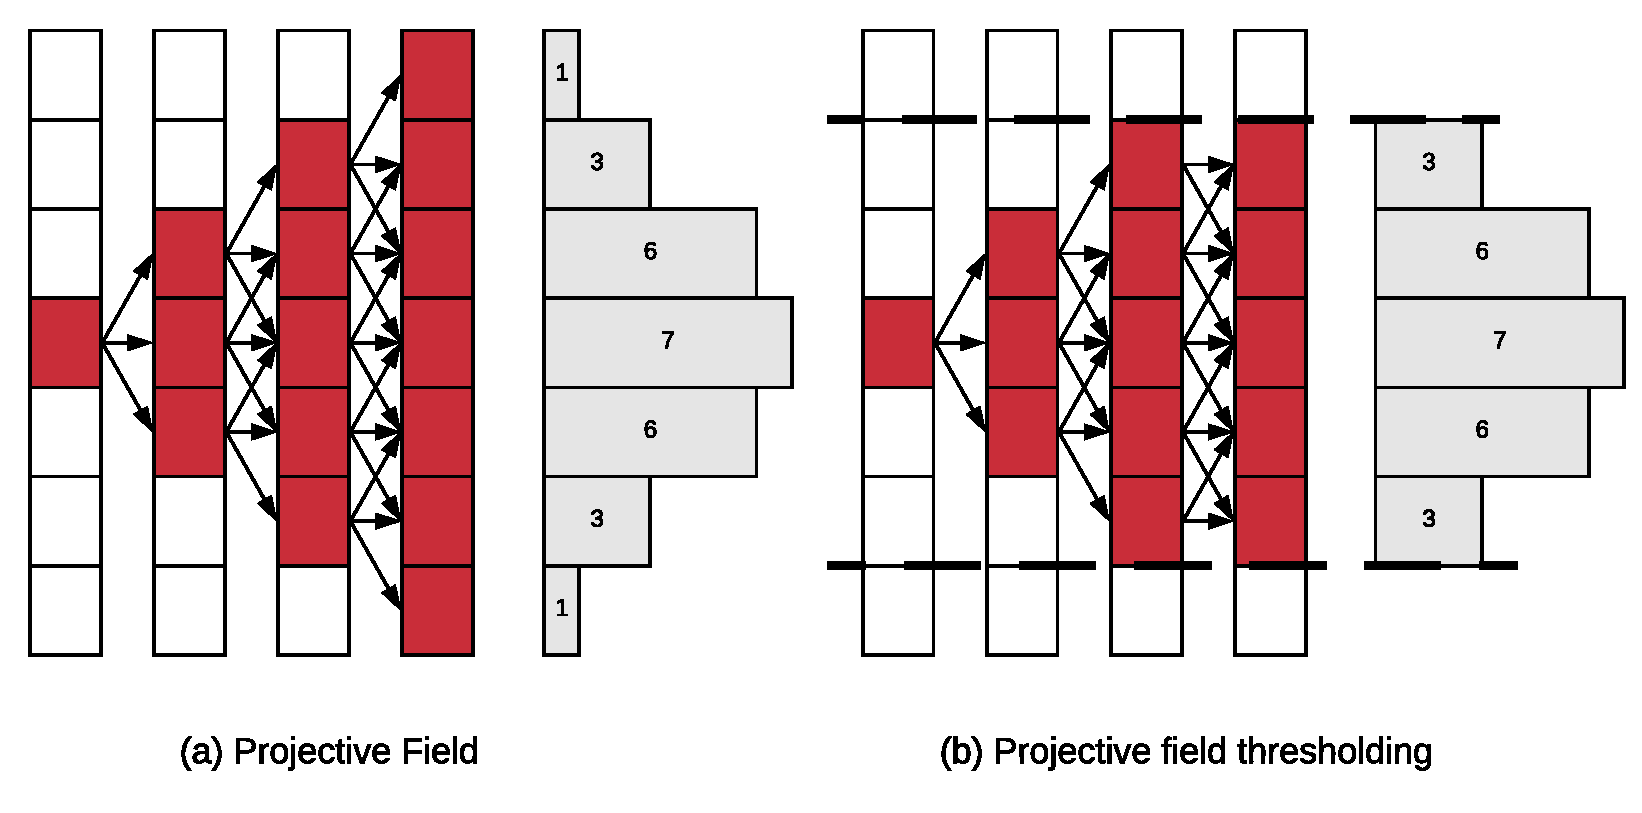
\includegraphics[width=\columnwidth]{images/pf_truncate}
\caption{(a) One dimensional Convolution demonstrating projective field growth (filter size = 2, stride = 1). (b) \textit{Projective field thresholding} with $\tau = 5/7$. Histograms denote the number of unique change propagation paths.}
\label{fig:pf_truncate}
\end{figure}

Because of the projective field growth, even though there will be much computational redundancies in the early layers, towards the latter layers it will decrease or even have no redundancies.
However, we empirically found that the projective field growth can be truncated up to a certain extent without significantly affecting the accuracy.
For a more intuitive understanding on why this would work consider the simplified one dimensional convolution example shown in Figure \ref{fig:pf_truncate} (a). In the example a single neuron is modified (marked in red) and a filter of size three is applied with a stride of one repeatedly four times.
Since the filter size is three, each updated neuron will propagate the change to three neurons in the next output layer causing the projective field to grow linearly.
At the end of the fourth layer, the histogram shows the number of unique paths that are available between each output neuron and the original updated neuron in the first layer.
It can be seen that this distribution resembles a Gaussian where many of the paths are connected to the central region.
The amount of actual change in the output layer is determined by both the number of unique paths and also the individual weights of the connections.
But the actual change in the output will converge to a Gaussian in distribution over all possible weight values.
For more details we refer the reader to \cite{luo2016understanding}, where a similar theoretical result has been proved for the receptive field\footnote{Receptive field of a CNN neuron is the local region (including the depth) of the input volume which is connected to it.} of a deep CNN.

As most of the change will be concentrated on the center, we introduce the notion of a projective field threshold $\tau ~ (0 < \tau \leq 1)$ which will be used to restrict the growth of the projective field.
It essentially determines the maximum size of the projective field as a fraction of the size of the output.
Figure \ref{fig:pf_truncate} (b) demonstrates the application of projective field thresholding with a $\tau$ value of $5/7$.
From the histogram generated for the projective field thresholding approach we can expect that much of the final output change will be maintained by this approach.

In \system, \textit{projective field thresholding} is implemented on top of \textit{incremental inference} approach by applying set of additional constraints on input-output coordinate mappings. For the horizontal dimension, the new set of calculations can be expressed as follows:

\begin{align}
\label{eqn:normal_width_calc}
W^\mathcal{O}_\mathcal{P} = &~ \texttt{min}\big(\lceil (W^\mathcal{I}_\mathcal{P} + W_\mathcal{K} - 1)/S_x \rceil, W^\mathcal{O}_\mathcal{P}\big)\\
\label{eqn:check_tau}
\text{If}~ W_\mathcal{P}^\mathcal{O} & > \texttt{round}(\tau \times W^\mathcal{O}):\\
\label{eqn:new_width_calc_with_tau}
& W^\mathcal{O}_\mathcal{P} = \texttt{round}(\tau \times W^\mathcal{O})\\
\label{eqn:new_in_width}
& W^\mathcal{I}_{\mathcal{P}_{new}} = W^\mathcal{O}_{\mathcal{P}} \times S_x - W_{\mathcal{K}} + 1\\
\label{eqn:new_x_coord}
& x^{\mathcal{I}}_\mathcal{P} \mathrel{+}= (W^\mathcal{I}_\mathcal{P} - W^\mathcal{I}_{\mathcal{P}_{new}})/2\\
\label{eqn:new_input_width}
& W^\mathcal{I}_{\mathcal{P}} = W^\mathcal{I}_{\mathcal{P}_{new}}\\
\label{eqn:new_output_x}
x^\mathcal{O}_\mathcal{P} = & \texttt{max}\big(\lceil (P_x + x^\mathcal{I}_\mathcal{P} - W_\mathcal{K} + 1)/S_x \rceil, 0\big)
\end{align}

Equation \ref{eqn:normal_width_calc} calculates output width assuming no thresholding. But if the output width exceeds the threshold defined by $\tau$, output width is set to the threshold value as per Equation \ref{eqn:new_width_calc_with_tau}.
Equation \ref{eqn:new_in_width} calculates the input width that would produce an output of width $W^\mathcal{O}_\mathcal{P}$ (think of this as making $W^{\mathcal{I}}_{\mathcal{P}}$ the subject of equation \ref{eqn:normal_width_calc}).
If the new input width is smaller than the original input width, the starting x coordinate should be updated as per Equation \ref{eqn:new_x_coord} such that the updated coordinates correspond to a center crop from the original.
Equation \ref{eqn:new_input_width} set the input width to the newly calculated input width and Equation \ref{eqn:new_output_x} calculates the x coordinate of the output patch from the updated values.
Coordinates and dimensions of the vertical dimension can also be computed similarly.


\begin{figure}[t]
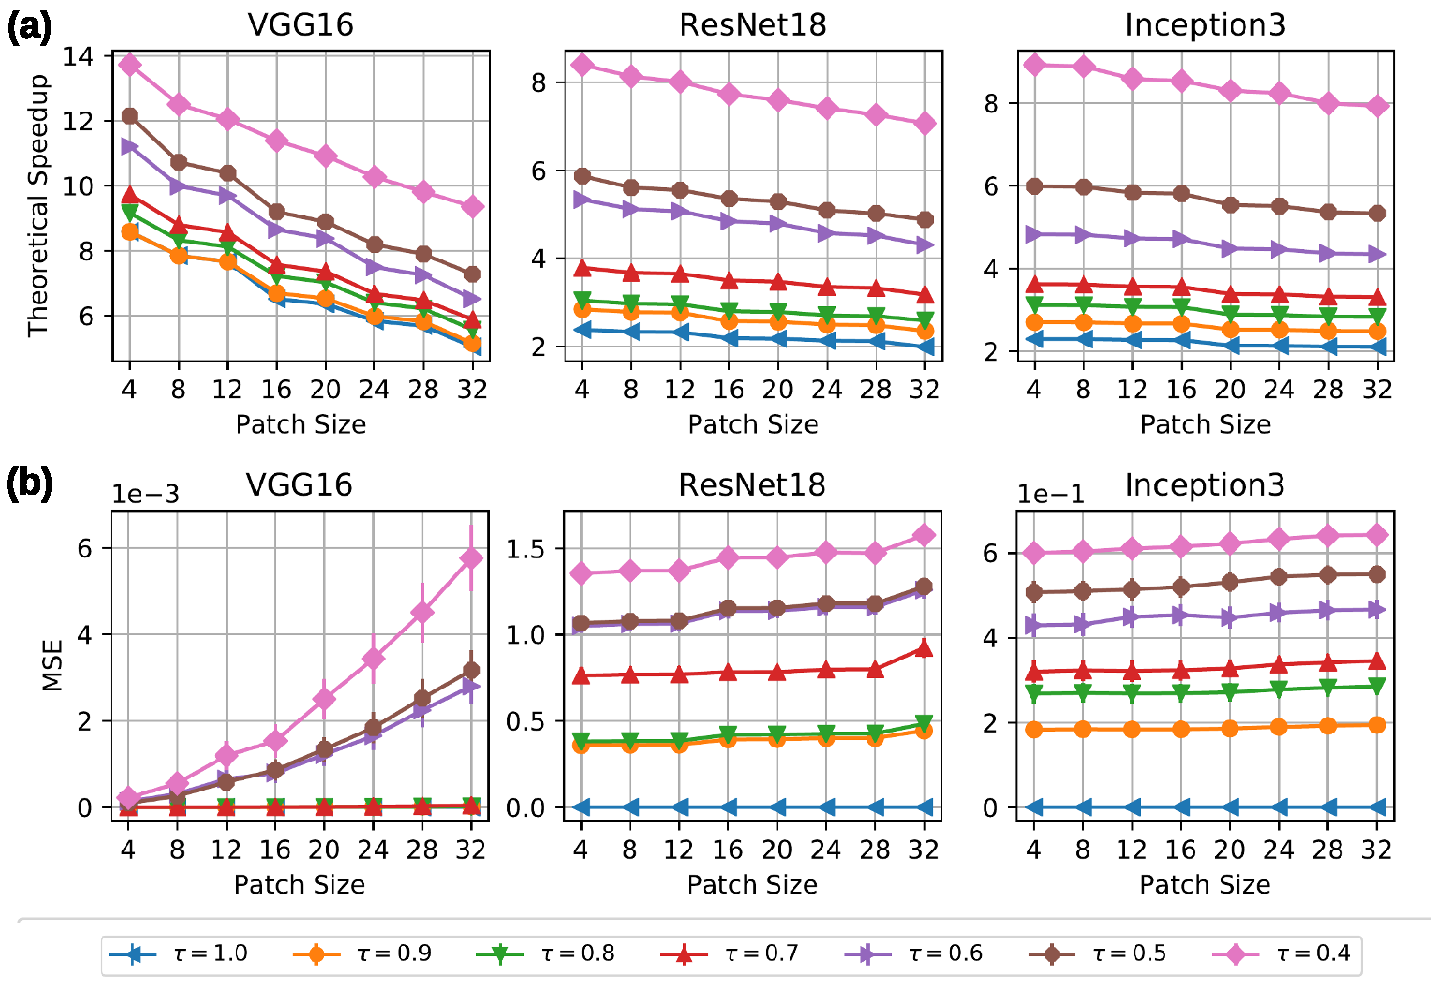
\includegraphics[width=\columnwidth]{images/proj_thresholding}
\caption{(a) Theoretical speedup ratio with projective field thresholding for different occlusion patch sizes and CNN models. (b) Mean Square Error between exact and approximate output of the final activation volume produce by a conv. or a pool layer for different occlusion patch sizes and CNN models on a sample (n=30) of OCT dataset. In both (a) and (b) occlusion patches are placed at the center of the image.}
\label{fig:th_redundancy_ratio}
\end{figure}


\subsection{Adaptive Drill-Down}\label{sec:ada-drill-down}
\textit{Adaptive drill-down} approach is based on the observation that in many occlusion based explainability workloads, such as in medical imaging, the regions of interest will occupy only a small fraction of the entire image.
In such cases it is unnecessary to inspect the entire image at a higher resolution with a small stride value for the occlusion patch.
In \textit{adaptive-drill-down} the final occlusion heatmap will be generated using a two stage process. At the first stage a low resolution heatmap will be generated by using a larger stride which we call stage one stride ($S_1$). From the heatmap generated at stage one, a predefined drill-down fraction ($r_{drill-down}$) of regions with highest probability drop for the predicted class is identified. At stage two, a high resolution occlusion map is generated using the original user provided stride value, also called stage two stride ($S_2$), only for the selected region. A schematic representation of \textit{adaptive drill-down} is shown in Figure \ref{fig:adaptive-drill-down}.

\begin{figure}[t]
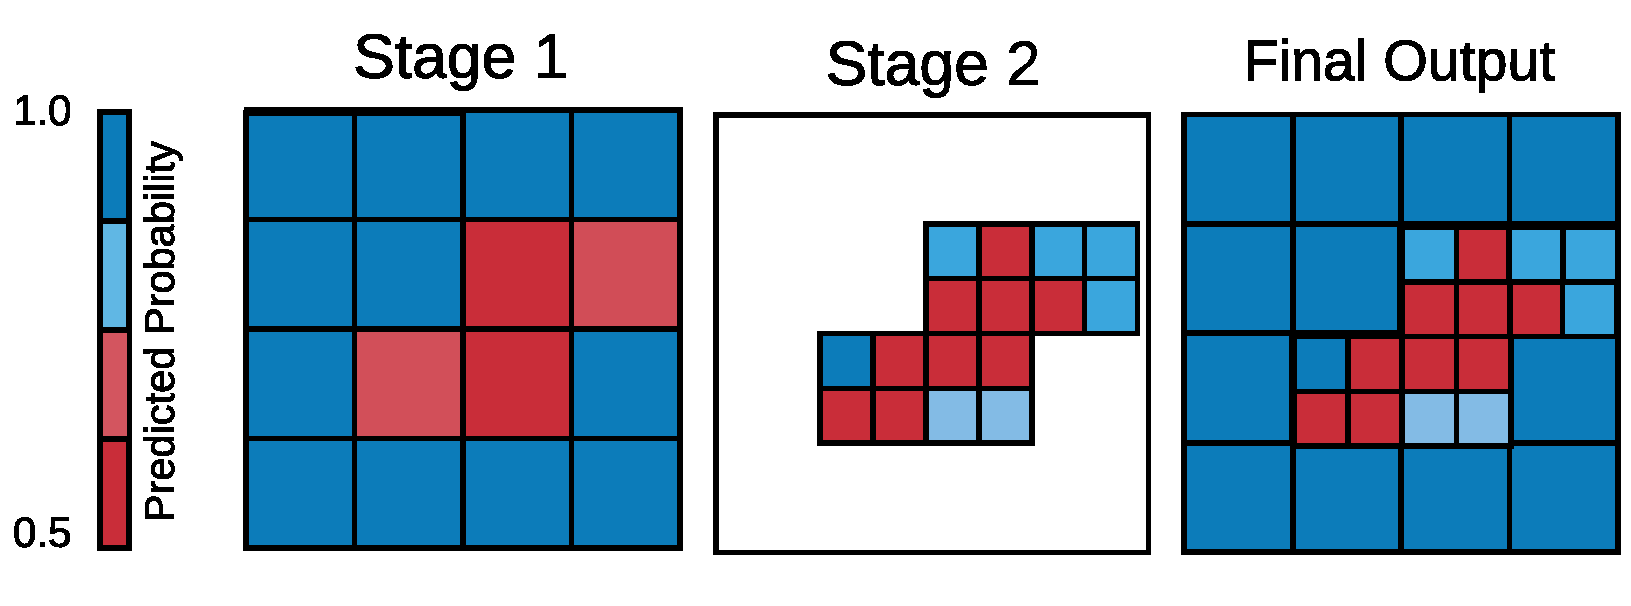
\includegraphics[width=\columnwidth]{images/adaptive-drill-down}
\caption{Schematic representation of \textit{adaptive drill-down}}
\label{fig:adaptive-drill-down}
\end{figure}

The amount of speedup that can be obtained from \textit{adaptive drill-down} is determined by both $r_{drill-down}$ and $S_1$.
If $r_{drill-down}$ is low, only a small region has to be examined at a higher resolution and thus will be faster.
However, this smaller region may not be sufficient to cover all the interesting regions on the image and hence can result in loosing important information.
Larger $S_1$ also reduces the overall runtime as it reduces the time taken for stage one. But it has the risk of mis-identifying interesting regions specially when the granularity of those regions is smaller than the occlusion patch size.
The speedup obtained by \textit{adaptive drill-down} approach is equal to the ratio between the number of individual occlusion patch positions generated for the normal and \textit{adaptive drill-down} approach.
Number of individual occlusion patch positions generated with a stride value of $S$ is proportional to $1/S^2$ (total number of patch positions is equal to $\frac{H_{\mathcal{I}_{img}}}{S} \times \frac{W_{\mathcal{I}_{img}}}{S}$).
Hence the speedup can  be expressed as per Equation \ref{eqn:addaptive-drill-down-eqn}.
Figure \ref{fig:r_and_s1} shows conceptually how the speedup would vary with $S_1$ when $r_{drill-down}$ is fixed and with $r_{drill-down}$ when $S_1$ is fixed.

\begin{align}
\label{eqn:addaptive-drill-down-eqn}
\texttt{speedup} = \frac{S^2_1}{S^2_2+r_{drill-down} \times S^2_1}
\end{align}

\begin{figure}[t]
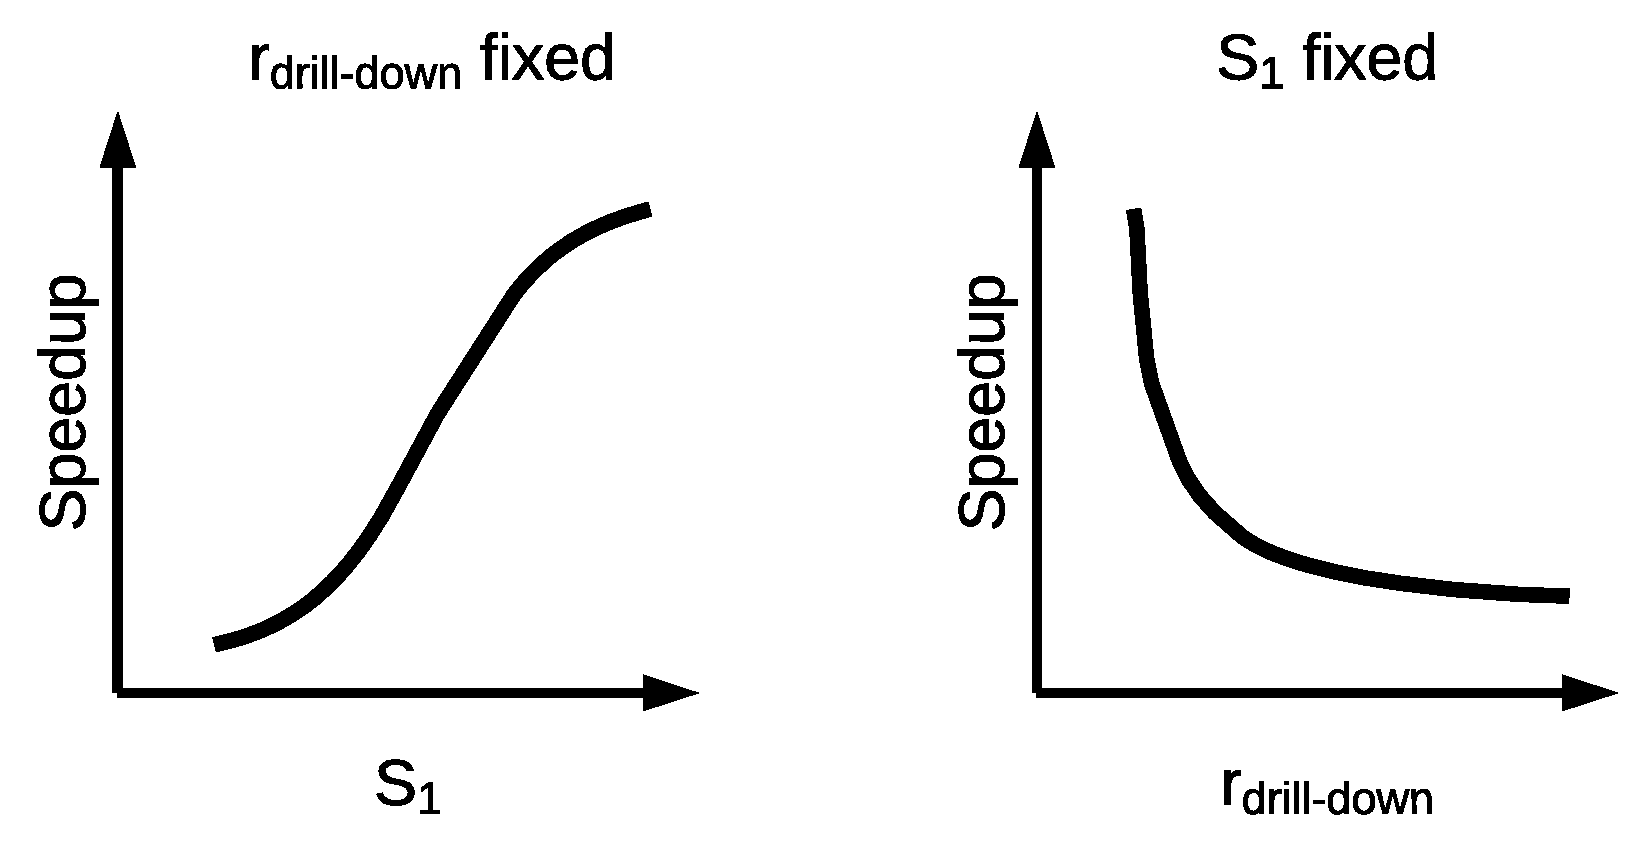
\includegraphics[width=0.7\columnwidth]{images/r_and_s1}
\caption{Conceptual diagram showing the effect of $S_1$ and $r_{drill-down}$ on speedup.}
\label{fig:r_and_s1}
\end{figure}

\subsection{System Tuning}
In this section we explain how \system~ sets it's internal configuration parameters for \textit{approximate inference} optimizations.

\vspace{2mm}
\noindent \textbf{Tuning projective field threshold.}
Tuning \textit{projective field threshold} ($\tau$) requires a special initial tuning phase.
During this tuning phase \system~ takes in a sample of images (default 30) from the operational workload and evaluates SSIM value of the approximate heatmap (compared to the exact heatmap) for different $\tau$ values (default values are 1.0, 0.9, 0.8, ..., 0.4).
These $\tau$ versus SSIM data points are then used to fit a second degree curve.
At operational time, \system~ requires the user to provide the expected level of quality for the heatmaps in terms of a SSIM value. $\tau$ is then selected from the curve fit to match this target SSIM value.
Figure \ref{fig:system_tuning} (a) shows the SSIM variation and degree two curve fit for different $\tau$ values and three different CNN models for a tuning set (n=30) from OCT dataset.
From the plots it can be seen that the distribution of SSIM versus $\tau$ lies in a lower dimensional manifold and with increasing $\tau$, SSIM also increases.
Figure \ref{fig:system_tuning} (b) shows the cumulative percentage plots for SSIM deviation for the tune and test sets (n=30) when the system is tuned for a target SSIM of 0.9.
For a target SSIM of 0.9 system picks $\tau$ values of 0.5, 0.7, and 0.9 for VGG16, ResNet18, and Inception3 models respectively.
It can be seen that approximately more than $50\%$ of test cases will result in an SSIM value of 0.9 or greater.
Even in cases where it performs worse than 0.9 SSIM, significant ($95\%-100\%$) portion of them are within +0.1 deviation.

\vspace{2mm}
\noindent \textbf{Tuning adaptive drill-down.}
As explained in section \ref{sec:ada-drill-down} the speedup obtained by \textit{adaptive drill-down} approach is determined by two factors, stage one stride value ($S_1$) and drill-down fraction ($r_{drill-down}$).
% Figure \ref{fig:adaptive_ssim} shows how the SSIM value of approximate heat maps would change when changing $r_{drill-down}$ and $S_1$ with all other configurations kept fixed.
% A general trend of increasing SSIM with increasing $r_{drill-down}$ and decreasing $S_1$ can be observed from the plots.
For configuring \textit{adaptive drill-down}, \system~ requires the user to provide $r_{drill-down}$ and a target \texttt{speedup} value.
$r_{drill-down}$ should be selected based on the user's experience and understanding on the relative size of interesting regions compared to the full image.
This is a fair assumption and in most cases, such as in medical imaging, users will have a fairly good understanding on the relative size of the interesting regions.
However, if the user is unable to provide this value, \system~ will use a default value, currently 0.25, as $r_{drill-down}$.
The \texttt{speedup} value basically captures user's input on how much faster the occlusion experiment should run.
Higher speedup values will sacrifice the quality of non-interesting (1-$r_{drill-down}$) regions for faster execution.
The default value for \texttt{speedup} value is three.
The way how \system~ configures \textit{adaptive drill-down} is different to how it configures \textit{projective field thresholding}.
The reason for this is, unlike in \textit{projective field thresholding}, in \textit{adaptive drill-down}, users have more intuition on the outcomes of $r_{drill-down}$ and target \texttt{speedup} compared to the SSIM quality value of the final output.
Given $r_{drill-down}$, target \texttt{speedup} value, and original occlusion patch stride value $S_2$ (also called stage two stride) \system~ then calculates the stage one stride value $S_1$ as per equation \ref{eqn:s1}.
As $S_1$ cannot be greater than the height ($H_{img}$) or width ($W_{img}$) of the image it can be seen that possible values for the \texttt{speedup} value are upper-bounded as per equation \ref{eqn:speedup_bound}.

\begin{align}
\label{eqn:s1}
S_1 = &~ \sqrt{\frac{\texttt{speedup}}{1 - r_{drill-down} \times \texttt{speedup}}} \times S_2
\end{align}

\begin{align}
\label{eqn:speedup_bound}
\begin{split}
S_1 = \sqrt{\frac{\texttt{speedup}}{1 - r_{drill-down} \times \texttt{speedup}}} \times S_2 < W_{img}\\
\texttt{speedup} < \frac{W^2_{img}}{S^2_2+r_{drill-down}\times W^2_{img}}
\end{split}
\end{align}


\begin{figure}[t]
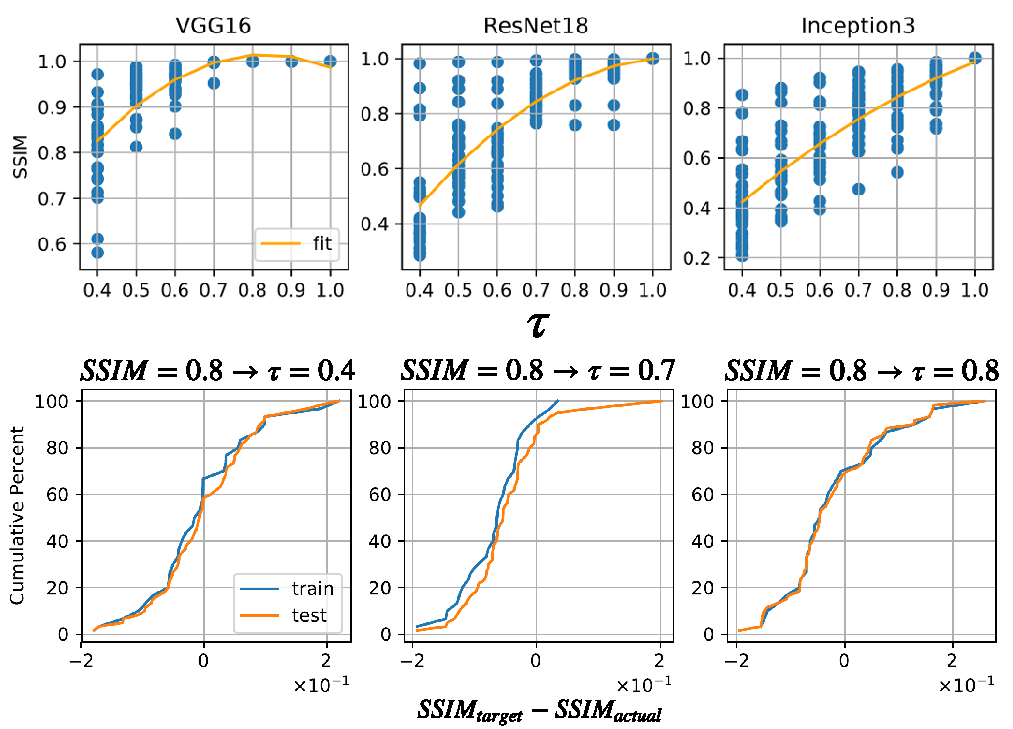
\includegraphics[width=\columnwidth]{images/system_tuning}
\caption{(a) SSIM variation and degree two curve fit for different $\tau$ values for a sample of OCT dataset. (b) Cumulative distribution plot for the SSIM deviation for the $\tau$ values obtained from the curve fit for a SSIM value of 0.9.}
\label{fig:system_tuning}
\end{figure}

% \begin{figure}[t]
% 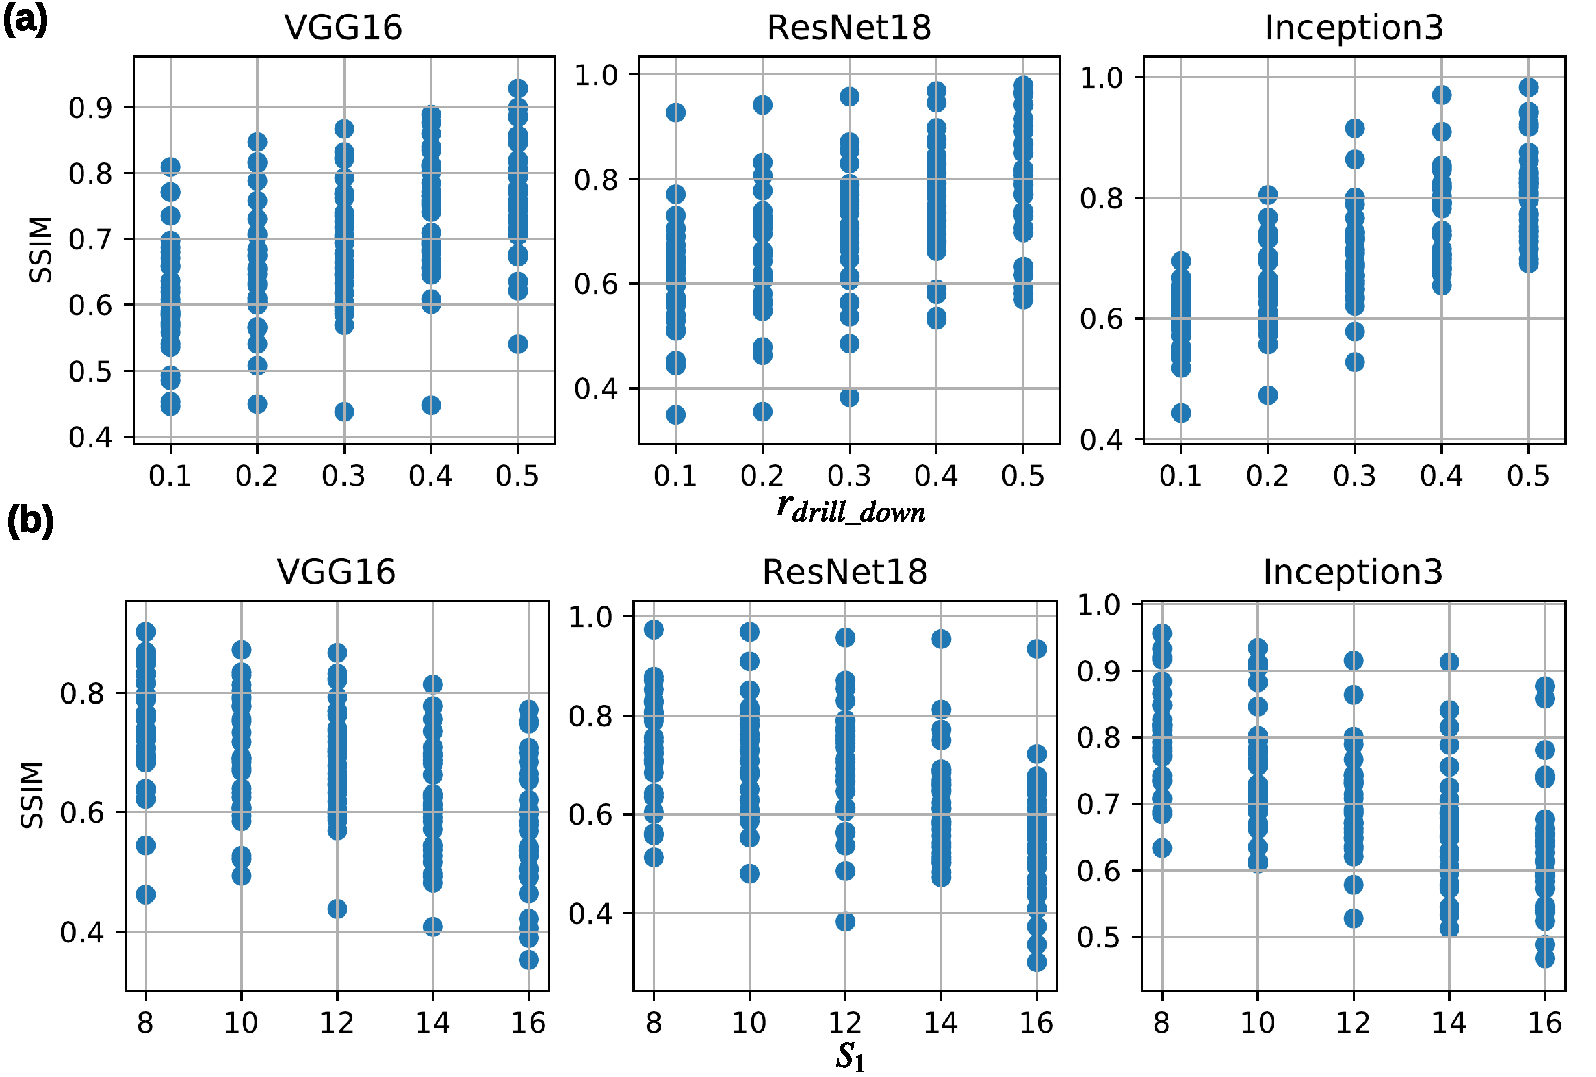
\includegraphics[width=\columnwidth]{images/adaptive_ssim}
% \caption{(a) SSIM variation for changing $r_{drill\_down}$ fixing $\tau=1$, $S_1=12$, and $S_2=4$. (b) SSIM variation for changing $S_1$ fixing $\tau=1.0$, $S_2=4$, and $r_{drill\_down}=0.3$ for a sample $(n=30)$ of OCT dataset.}
% \label{fig:adaptive_ssim}
% \end{figure}

